\documentclass[12pt,a4paper]{article}

%\usepackage[left=1.5cm,right=1.5cm,top=1cm,bottom=2cm]{geometry}
\usepackage[in, plain]{fullpage}
\usepackage{array}
%\usepackage{../../pas-math}
\usepackage{../../moncours}



%-------------------------------------------------------------------------------
%          -Packages nécessaires pour écrire en Français et en UTF8-
%-------------------------------------------------------------------------------
\usepackage[utf8]{inputenc}
\usepackage[frenchb]{babel}
%\usepackage{numprint}
\usepackage[T1]{fontenc}
%\usepackage{lmodern}
\usepackage{textcomp}
\usepackage[french, boxed]{algorithm2e}
\usepackage{hyperref}


%-------------------------------------------------------------------------------

%-------------------------------------------------------------------------------
%                          -Outils de mise en forme-
%-------------------------------------------------------------------------------
\usepackage{hyperref}
\hypersetup{pdfstartview=XYZ}
%\usepackage{enumerate}
\usepackage{graphicx}
\usepackage{multicol}
\usepackage{tabularx}
\usepackage{multirow}
\usepackage{color}
\usepackage{eurosym}


\usepackage{anysize} %%pour pouvoir mettre les marges qu'on veut
%\marginsize{2.5cm}{2.5cm}{2.5cm}{2.5cm}

\usepackage{indentfirst} %%pour que les premier paragraphes soient aussi indentés
\usepackage{verbatim}
\usepackage{enumitem}
\usepackage{booktabs}
\usepackage[usenames,dvipsnames,svgnames,table]{xcolor}

\usepackage{variations}

%-------------------------------------------------------------------------------


%-------------------------------------------------------------------------------
%                  -Nécessaires pour écrire des mathématiques-
%-------------------------------------------------------------------------------
\usepackage{amsfonts}
\usepackage{amssymb}
\usepackage{amsmath}
\usepackage{amsthm}
\usepackage{tikz}
\usepackage{xlop}
\usepackage[output-decimal-marker={,}]{siunitx}
%-------------------------------------------------------------------------------

%-------------------------------------------------------------------------------
%                  -Nécessaires pour écrire des formules chimiquess-
%-------------------------------------------------------------------------------

\usepackage[version=4]{mhchem}

%-------------------------------------------------------------------------------
% Pour pouvoir exploiter les fichiers directement dans beamer
\newcommand{\pause}{\ }
%-------------------------------------------------------------------------------
%                    - Mise en forme avancée
%-------------------------------------------------------------------------------

\usepackage{ifthen}
\usepackage{ifmtarg}


\newcommand{\ifTrue}[2]{\ifthenelse{\equal{#1}{true}}{#2}{$\qquad \qquad$}}

%\newcommand{\kword}[1]{\textcolor{red}{\underline{#1}}}
%-------------------------------------------------------------------------------

%-------------------------------------------------------------------------------
%                     -Mise en forme d'exercices-
%-------------------------------------------------------------------------------
%\newtheoremstyle{exostyle}
%{\topsep}% espace avant
%{\topsep}% espace apres
%{}% Police utilisee par le style de thm
%{}% Indentation (vide = aucune, \parindent = indentation paragraphe)
%{\bfseries}% Police du titre de thm
%{.}% Signe de ponctuation apres le titre du thm
%{ }% Espace apres le titre du thm (\newline = linebreak)
%{\thmname{#1}\thmnumber{ #2}\thmnote{. \normalfont{\textit{#3}}}}% composants du titre du thm : \thmname = nom du thm, \thmnumber = numéro du thm, \thmnote = sous-titre du thm

%\theoremstyle{exostyle}
%\newtheorem{exercice}{Exercice}
%
%\newenvironment{questions}{
%\begin{enumerate}[\hspace{12pt}\bfseries\itshape a.]}{\end{enumerate}
%} %mettre un 1 à la place du a si on veut des numéros au lieu de lettres pour les questions 
%-------------------------------------------------------------------------------

%-------------------------------------------------------------------------------
%                    - Mise en forme de tableaux -
%-------------------------------------------------------------------------------

\renewcommand{\arraystretch}{1.7}

\setlength{\tabcolsep}{1.2cm}

%-------------------------------------------------------------------------------



%-------------------------------------------------------------------------------
%                    - Racourcis d'écriture -
%-------------------------------------------------------------------------------
%Droites
\newcommand{\dte}[1]{$(#1)$}
\newcommand{\fig}[1]{figure $#1$}
\newcommand{\sym}{symétrique}
\newcommand{\syms}{symétriques}
\newcommand{\asym}{axe de symétrie}
\newcommand{\asyms}{axes de symétrie}
\newcommand{\seg}[1]{$[#1]$}
\newcommand{\monAngle}[1]{$\widehat{#1}$}
\newcommand{\bissec}{bissectrice}
\newcommand{\mediat}{médiatrice}
\newcommand{\ddte}[1]{$[#1)$}


% Angles orientés (couples de vecteurs)
\newcommand{\aopp}[2]{(\vec{#1}, \vec{#2})} %Les deuc vecteurs sont positifs
\newcommand{\aopn}[2]{(\vec{#1}, -\vec{#2})} %Le second vecteur est négatif
\newcommand{\aonp}[2]{(-\vec{#1}, \vec{#2})} %Le premier vecteur est négatif
\newcommand{\aonn}[2]{(-\vec{#1}, -\vec{#2})} %Les deux vecteurs sont négatifs

%Ensembles mathématiques
\newcommand{\naturels}{\mathbb{N}} %Nombres naturels
\newcommand{\relatifs}{\mathbb{Z}} %Nombres relatifs
\newcommand{\rationnels}{\mathbb{Q}} %Nombres rationnels
\newcommand{\reels}{\mathbb{R}} %Nombres réels
\newcommand{\complexes}{\mathbb{C}} %Nombres complexes


%Intégration des parenthèses aux cosinus
\newcommand{\cosP}[1]{\cos\left(#1\right)}
\newcommand{\sinP}[1]{\sin\left(#1\right)}


%Probas stats
\newcommand{\stat}{statistique}
\newcommand{\stats}{statistiques}


\newcommand{\homo}{homothétie}
\newcommand{\homos}{homothéties}


\newcommand{\mycoord}[3]{(\textcolor{red}{\num{#1}} ; \textcolor{Green}{\num{#2}} ; \textcolor{blue}{\num{#3}})}
%-------------------------------------------------------------------------------

%-------------------------------------------------------------------------------
%                    - Mise en page -
%-------------------------------------------------------------------------------

\newcommand{\twoCol}[1]{\begin{multicols}{2}#1\end{multicols}}


\setenumerate[1]{font=\bfseries,label=\textit{\alph*})}
\setenumerate[2]{font=\bfseries,label=\arabic*)}


%-------------------------------------------------------------------------------
%                    - Elements cours -
%-------------------------------------------------------------------------------

%Correction d'exercice
\newcommand{\exoSec}[2]{\subsection*{Exercice #1 page #2}}
%-------------------------------------------------------------------------------
%                    - raccourcis d'écriture -
%-------------------------------------------------------------------------------

%Mise en évidence de termes clés
\newcommand{\mykw}[1]{\textcolor{red}{\underline{\textbf{#1}}}}

%Exercices
\newcommand{\exo}[2]{exercice #1 page #2}
\newcommand{\Exo}[2]{Exercice #1 page #2}

\renewcommand{\pause}{\ }

\graphicspath{{./img/}}


\date{}
\title{}


\begin{document}
	
	
\chap[num=5, color=blue]{{Puissance d'un appareil électrique}}{\today }	


%\section{Comment caractériser un mouvement ?}

\begin{questions}
	\question Le mouvement du tunnelier est \underline{rectiligne} et \underline{uniforme}.
	
	\question Lors du fonctionnement du tunnelier, la roue coupante a une trajectoire \underline{circulaire}.
	
	\question Lors d'un cycle de fonctionnement du tunnelier la roue :
	\begin{enumerate}
		\item commence par démarrer, donc sa vitesse augmente ;
		\item puis elle se stabilise à vitesse constante;
		\item enfin elle ralenti pour s'arrêter.
	\end{enumerate} 

	\question La roue coupante du tunnelier a donc un mouvement :
	\begin{enumerate}
		\item d'abord circulaire accéléré;
		\item ensuite circulaire uniforme;
		\item enfin circulaire ralenti;
	\end{enumerate} 
\end{questions}

\section{Puissance électrique}
%\section[Conservation de la masse lors d'une transformation  chimique]{\texorpdfstring{Conservation de la masse lors d'une transformation \\ chimique}{Conservation de la masse lors d'une transformation  chimique}}

%\begin{frame}
%	\begin{myact}{}

		Activité 16 page 51 cahier d'activités

\end{myact}
%\end{frame}
\begin{mybilan}
	\begin{itemize}
		\item La \kw{fiche signalétique} d'un appareil électrique indique sa tension nominale (en volts, $V$) et sa puissance de fonctionnement ()en watt, $W$).
		\item L'énergie électrique fournie par le secteur est \kw{convertie} en un autre type d'énergie suivant l'objet utilisé. \'Energie thermique pour un appareil de chauffage, énergie lumineuse pour une lampe, etc.
		\item Toute l'énergie apportée à l'appareil est convertie, il y a \kw{conservation de l'énergie}. L'énergie apportée est égale à la somme des énergies fournies par l'appareil.
	\end{itemize}
	
	
\end{mybilan}




\begin{myex}
	\begin{itemize}
		\item Fiche signalétique d'un appareil électrique
		
		\begin{center}
			\includegraphics[scale=0.7]{fiche}
		\end{center}
		
		\item Chaîne énergétique d'un dispositif d'éclairage
		
		\begin{center}
			\includegraphics[scale=0.4]{chaine}
		\end{center}
	\end{itemize}

	
\end{myex}


\section{Puissance, tension et intensité}


\begin{mybilan}
	\begin{itemize}
		\item Dans le système international, la puissance est exprimée en \kw{watt, notée W}.
		\item La puissance $P$ d'un appareil électrique dépend de sa tension de fonctionnement $U$ et de l'intensité du courant reçu $I$. On a: 
		\begin{equation*}
			P = U \times I
		\end{equation*}
	avec $P$ en watt ($W$), $U$ en volts ($V$) et $I$ en ampère ($A$).
	\end{itemize}
		
		 
\end{mybilan}


\begin{myex}
	Ordres de grandeur de puissance :
	\begin{center}
		\includegraphics[scale=0.4]{ordre}
	\end{center}
\end{myex}

\section{\'Energie électrique}

\begin{mybilan}

	L'\kw{énergie électrique} utilisée par un appareil de puissance $P$ qui fonctionne pendant une durée $t$ est donné par la relation :
	\begin{equation*}
		E = P \times t
	\end{equation*}
	Avec $E$ en kilowattheure (kWh), $P$ en kilowatt (kW) et $t$ en heures (h), ou  $E$ en joules (J), $P$ en watt (W) et $t$ en secondes (s).\\

	Utiliser des appareil électriques moins puissants, diminuer leur durée de fonctionnement et éviter de les laisser en veille réduit la consommation d'énergie électrique.
 
\end{mybilan}

\begin{myrem}
	Le joule est une unité très petite, dans la pratique, on utilise le kilowattheure.

	\begin{equation*}
		1 kWh = 1 kW \times 1h = 1000 W \times 3600 s = \num{3.6} \times 10^{6} J
	\end{equation*}
\end{myrem}


\begin{center}
	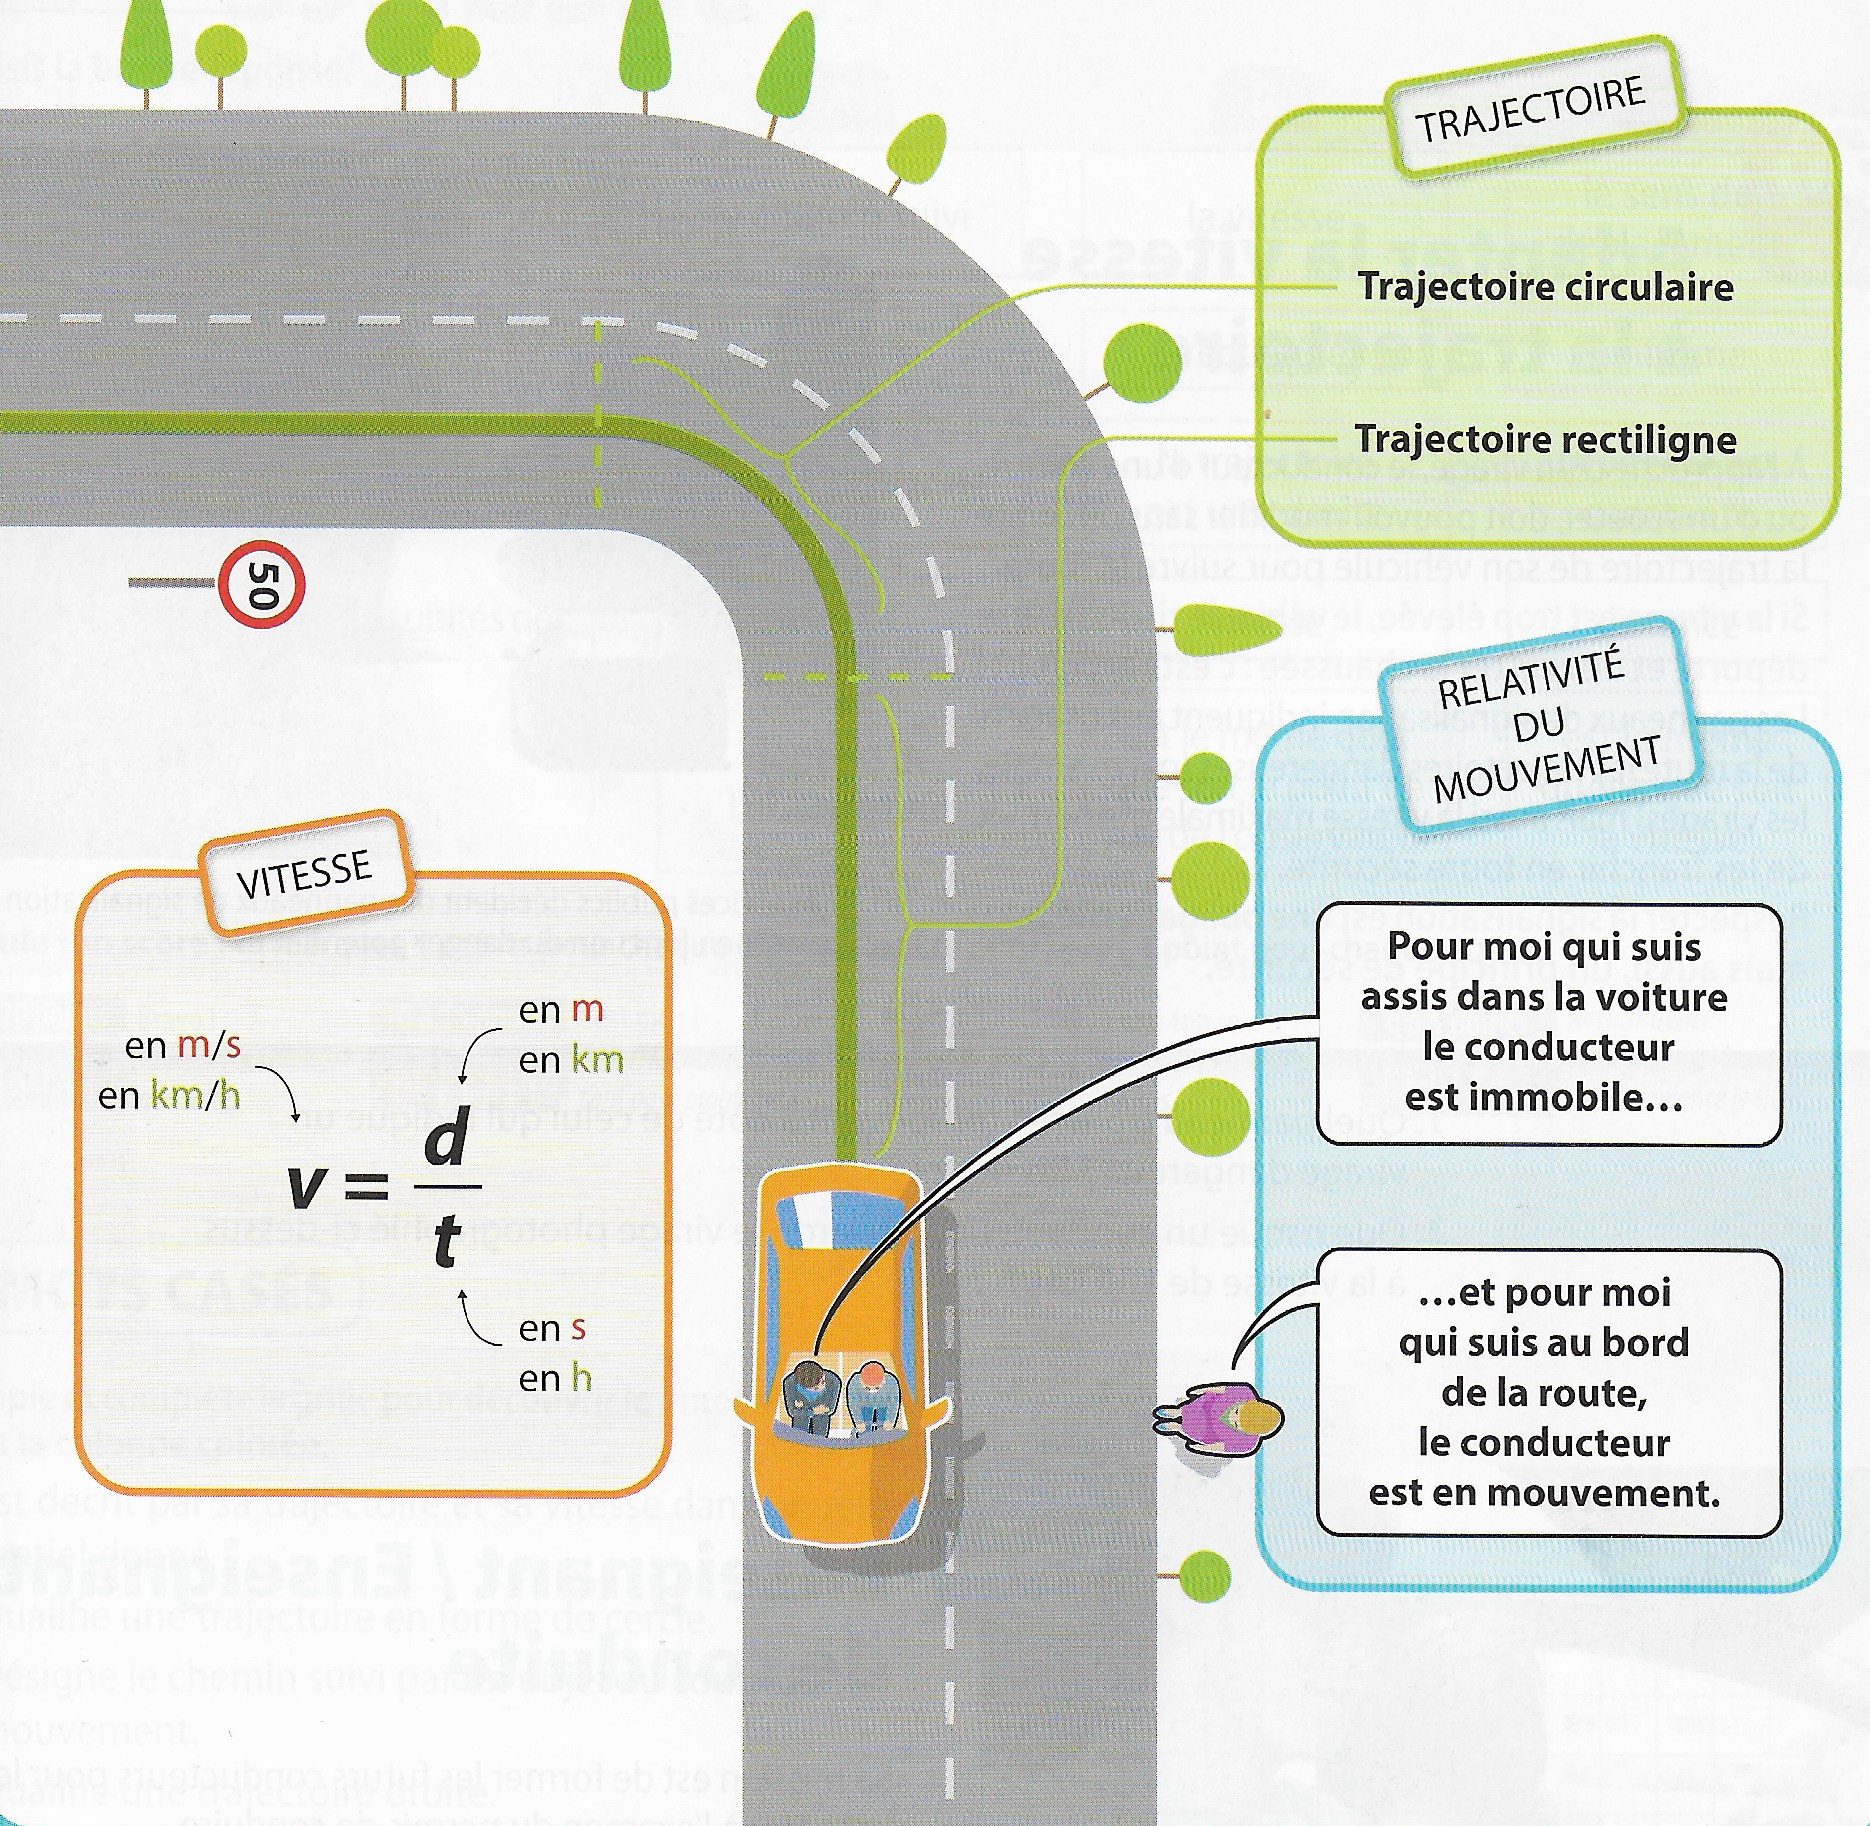
\includegraphics[scale=0.3]{bilan}
\end{center}
\end{document}